\chapter{Test on EEG measurements}\label{ch:eeg_test}
The main algorithm was implemented and tested on simulated data in chapter \ref{ch:implementation}. 
In this chapter the main algorithm is tested on EEG measurements, for which it is intended. 
Two different approaches are consider with respect to evaluating the resulting estimates of the source signals -- ICA comparison and alpha wave analysis, respectively.

At first the provided data sets with EEG measurements are described. Followed by a test description and an analysis of the results for both of the evaluation approaches. 
Finally, a summary is provided to highlight the conclusions.  

\section{Data Description}
For this thesis a data base of real EEG scalp measurements has been provided, from the the department of .... at AAU \todo{Indsæt department - L}. 
The data base consist of data sets of EEG measurements resulting from three test subjects. 
For each of three test subjects two data set is provided, one where the test subject sit still with open eyes and one similar but with closed eyes, resulting in a data base with 6 data sets.  
For the measurements an EEG cap with $32$ sensors measuring the scalp EEG signal with sample frequency at $512$Hz\todo{tjek sample frequency ant time} over a period of $XX$ seconds, resulting in $L = XX$ samples. 
That is 27 channels with names and position available in \texttt{EEG.chanlocs} structure \todo{Matlab eller python her?}.   

Before the data base was provided each raw data set had undergone the following preprocessing.
The data was bandpass filtered between 1 and 40 Hz. Then decomposed by ICA where the independent components related to eye activity or movement was removed. Thus, for every data set 27 sensors remains. One data set then consist solely of the measurement matrix $\mathbf{Y} \in \mathbb{R}^{27\times ??}$.

%The data set is then ready to be divided in segments for which a source matrix $\hat{\textbf{X}}$ is to be estimated by the main algorithm described in chapter \ref{ch:implementation}.

\section{Test Description}
The test procedure is now described through specification of the evaluation criteria and the practical implementation of the test.
Remember that the aim of the developed main algorithm is to estimated the source matrix in the case where the number of sensors is less than the number of active source signals -- $M<k\leq N$.

\subsection{Performance Evaluation by Comparison to ICA}
From the description of ICA used on EEG measurements, cf. section \ref{sec:ICAsolution} ICA are considered unreliable when using low-density EEG equipment where $M<32$, but for $M \geq 32$ the currently considered the most reliably method for the source estimation. However note again that the true number of sources is not known thus there is always some unreliability to the result. 

From the view that the sources found by ICA where $N=M$ is the best estimate, it is possible to let that estimate serve as a reference to be compared to the estimates achieved when $M<N$. 
In practice that is to perform ICA on a data set $\textbf{Y} \in \mathbb{R}^{M \times L}$ resulting in $\hat{\textbf{X}}_{ICA}\in \mathbb{R}^{N\times L}$ where $M=N$. 
Then a specific number of sensors are removed from the data set $\textbf{Y}$ such that $M<N$ then and $\hat{\textbf{X}}_{Main}\in \mathbb{R}^{N\times L}$ is estimated by the main algorithm. 
Then the performance of the main algorithm can be measured by comparison to the $\hat{\textbf{X}}_{ICA}$ -- does the main algorithm manage to find the same active sources as ICA, but for $M<N$?

In appendix \ref{app:ica_test} the ICA algorithm is verified on simulated data without noise. 
It is found that ICA manage to estimate $\textbf{X}$ almost exact, when $M=N=k$. 
Furthermore, it is seen that for $k < N$ ICA manage to estimate the zero rows as zero. This supports that the estimate by ICA can serve as a reference.     

To compare the two estimates the MSE, cf. section \ref{sec:mse}, is used. 
However, an issue arise due to the fact that ICA do not manage to localise each of the found sources. 
That is the row of $\hat{\textbf{X}}_{ICA}$ do not correspond to the true $\textbf{X}$. 
Furthermore, the ICA algorithm is invariant toward phase and amplitude. This must necessarily worsen the resulting MSE.  

The issue is cover in appendix \ref{app:ica_test}. 
Here a function is considered, which manage to pair and fit the rows with the lowest mutual MSE an then arrange the rows of $\hat{\textbf{X}}_{ICA}$ such that $MSE(\textbf{X},\hat{\textbf{X}}_{ICA})$ is minimised. 
The fitting consist of a possible phase shift and scaling of the the amplitude. 
The right optimal fit was found through a brute-force search, however this is not possible as the possible number of combinations increases as $k$ increases. 
This suggest the definition of an optimisation problem minimising the resulting MSE with respect to the combination of row indexes, possible phase and corresponding amplitude scaling. 
unfortunately an successful optimization was not achieved within the time scope of this project, thus the fitting process is not applied to the results achieved from the EEG measurements in this chapter. 
This factor must be taken into account when evaluating the results.    

Consider again the resulting $MSE(\hat{\textbf{X}}_{ICA},\hat{\textbf{X}}_{Main})$. 
To evaluate further on the question whether the same sources have been found a tolerance for the MSE is introduced. 
With $MSE(\hat{\textbf{X}}_{ICA},\hat{\textbf{X}}_{Main})$ being an average over the MSE of each row within one segment a low value indicate that main part of the rows makes an estimate similar the estimate from ICA. 
From this perspective a tolerance for $MSE(\hat{\textbf{X}}_{ICA},\hat{\textbf{X}}_{Main})$ decides whether the same sources are achieved with success. 
The tolerance is set to 6 due to previous observations with respect to the simulated data, especially figure \ref{fig:AR2} indicate that an MSE below 6 is achievable for a system where $M<<N$ with use of $\textbf{A}_real$. 
It could be argued that the tolerance should be increased as the estimate of $\textbf{A}$ is not expected to be nearly as good, however this will could give a distorted image of the results.          

\subsection{Test Setup}
The test set up is visualised in figure \ref{fig:flow2} by a flow diagram, showing the essential steps of the test. 
\begin{figure}[H]
    \centering
	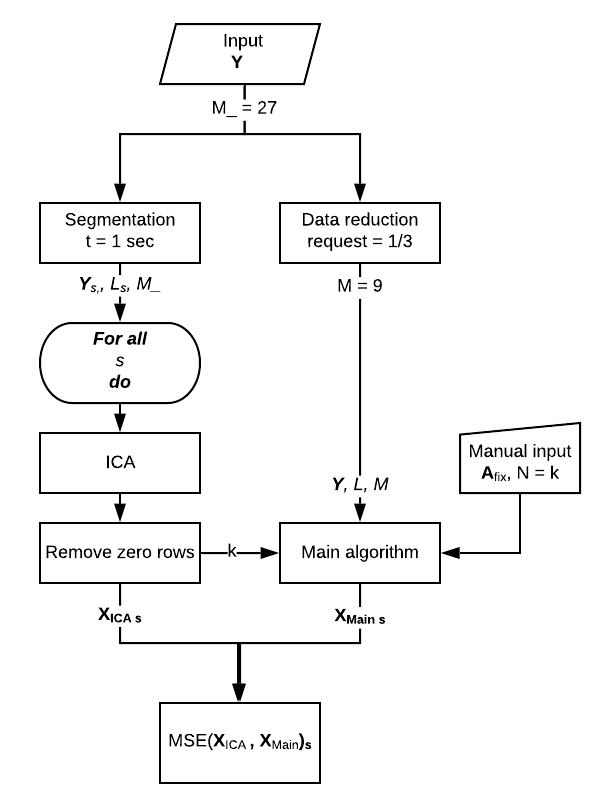
\includegraphics[scale=1]{figures/ch_7/flow2.png}
	\caption{Flow diagram for visualisation of the test procedure for one data set. Example given for $M<N$ where \texttt{request = 1/3} result in $M=9$.}
	\label{fig:flow2}
\end{figure}
\todo{inset hat over X on figure}
%%% describtion of the flowchart - remainings
In the flow diagram the two estimation processes are seen to run parallel but taking the same input. 
Prior to the application of ICA the input is divided into segments. 
That is the same segmentation as inside the main algorithm, cf. section \ref{sec:implementation_flow}.
The size of the segments are defined due to the expected stationarity of the sources. 
As described in the motivation chapter \ref{ch:motivation} sources are stationary if you look at sufficiently small intervals. 
Segments at $t = 1$ second is chosen from the belief that the brain activity can be assumed stationary with in short time interval.
Furthermore, one must take in mind that shorter time interval lead to more segments and therefore a higher computational complexity.   
After the segmentation the ICA is applied to every segment, returning $\hat{\textbf{X}}_{ICA s} \in \mathbb{R}^{M \times L_s}$.
From appendix \ref{app:ica_test} it is seen that ICA manage to estimate the non-active sources by zero rows, when no noise is present. 
When ICA is applied to the EEG measurements noise is expected. 
Thus the non-active sources defined by the average amplitude being within a tolerance interval around zero, defined by tol = $[10E-03, -10E-03]$. 
When the non-active sources are identified they are removed and the resulting estimate is reduced to $\hat{\textbf{X}}_{ICA s} \in \mathbb{R}^{k \times L_s}$. 
The found number of active sources $k$ is then given as input to the main algorithm where $k = N$. 
In parallel to the ICA process the input data is reduced as specified in the previous subsection. 
Then the main algorithm is applied to the reduced data set. 
Within the main algorithm the data is like wise divided in segments and an estimate $\hat{\textbf{X}}_{Main s} \in \mathbb{R}^{k \times L_s}$ is returned. 
Note that $\textbf{A}_{fix}$ is given as a manual input, replacing the COV-DL algorithm as concluded in chapter \ref{ch:implementation}.
At the end the resulting two estimates have the same dimensions which allows for $\hat{\textbf{X}}_{Main s}$ to be evaluated with respect to $\hat{\textbf{X}}_{ICA s}$ by the MSE.            
\\ \\
The described test is performed on the following three cases,
\begin{itemize}
\item \textbf{Case 0}: $M = N$ , to see the best possible result achieved by the main algorithm. 
\item \textbf{Case 1}: $M < N$ every third sensor is removed. 
\item \textbf{Case 2}: $M << N$ every second sensor is removed.
\end{itemize}

\section{Results}
For each case the test is performed on three data set -- \texttt{S1\_Cclean}, \texttt{S2\_Cclean} and \texttt{S3\_Cclean}. Measurements for three test subjects sitting with closed eyes in $??$ seconds.
The results is plotted for one data set for visual understanding, lastly the results of all three data sets are compared in a table.  

\subsection{Case 0, $M = N$}
ICA is applied on $\mathbf{Y}_s$ specified by $M\_ = 27$ and $L_s = 516$. 
The main algorithm is applied on $\mathbf{Y}_s$ without any reduction hence specified by $M = 27$ and $L_s = 516$, given $\hat{\mathbf{A}}_{\text{fix}}$ and $N = k$ provided from ICA.
Figure \ref{fig:M=N_1} show $\text{MSE}\left(\hat{\mathbf{X}}_{\text{main}},\hat{\mathbf{X}}_{\text{ICA}}\right)$ for all segments $s$. 
Figure \ref{fig:M=N_1_2} show the same plot but the y-axis is specified to the interval $[-10,50]$ for better visualization.
Furthermore, the MSE tolerance $= 5$ is visualized, indicting for each segment whether the estimate $\hat{\mathbf{X}}_{\text{main}}$ is sufficiency close to $\hat{\mathbf{X}}_{\text{ICA}}$. 
For a majority of the segments the MSE lies under the tolerance, but single outliers appears for which the MSE of the segment is significantly increased. Taking the average over all segments the average achieved MSE is $5.17$.    
\begin{figure}[H]
\begin{widepage}
    \begin{minipage}[t]{.45\textwidth}
		\centering
		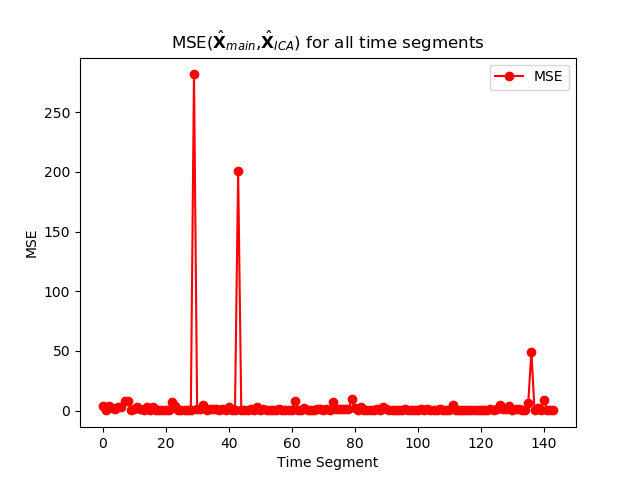
\includegraphics[width=1\linewidth]{figures/ch_7/resultat/average_mse_none_removed_ica}
	\caption{$\text{MSE} \left(\hat{\mathbf{X}}_{\text{main}}, \hat{\mathbf{X}}_{\text{ICA}}\right)$ for all $n_{\text{seg}} = $ 144 segments.}
	\label{fig:M=N_1}
    \end{minipage} 
    \hspace{0.5cm}
    \begin{minipage}[t]{.45\textwidth}
        \centering
		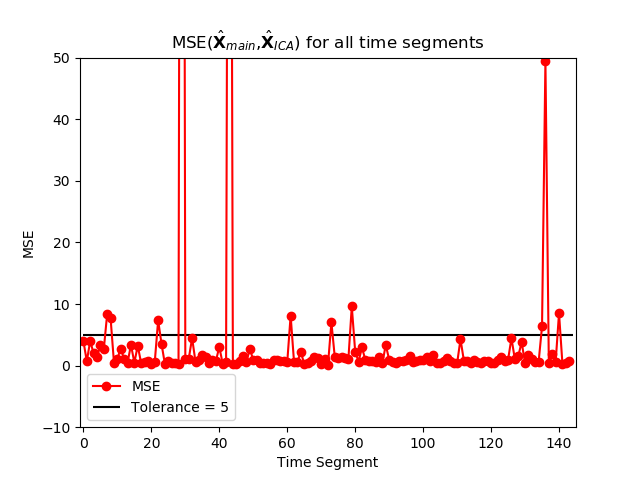
\includegraphics[width=1\linewidth]{figures/ch_7/resultat/average_mse_none_removed_ica_zoom.png}
	\caption{$\text{MSE} \left(\hat{\mathbf{X}}_{\text{main}}, \hat{\mathbf{X}}_{\text{ICA}}\right)$ for all $n_{\text{seg}} = $ 144 segments. Visualized only for the y-axis interval $[-10, 50]$ for better visualization.}
	\label{fig:M=N_1_2}
    \end{minipage}
\end{widepage}
\end{figure}
\noindent
To investigate the behavior of a single segment figure \ref{fig:M=N_2} show the MSE value computed for each row of the two estimates of a specific segment. 
That is MSE$(\hat{\mathbf{X}}_{\text{main}_{i}}$, $\hat{\mathbf{X}}_{\text{ICA}_{i}})$ for every row $i = 1, \dots, k$ in time segment $s = 5$. 
Additionally figure \ref{fig:M=N_3} show and compare the corresponding estimates for four random chosen sources. 
This allows for visual comparison of the estimates relative to the corresponding MSE value seen in figure \ref{fig:M=N_2}. 
Note that for better visual comparison each visualized row of $\hat{\mathbf{X}}_{\text{ICA}}$ is scaled with respect to the max value of the corresponding row in $\hat{\mathbf{X}}_{\text{main}}$.
From figure \ref{fig:M=N_2} it is seen that the estimate of each source result in a relative low MSE. This indicates that the main algorithm has managed to estimate the same source as the ICA algorithm. 
In contradiction to this, figure \ref{fig:M=N_3} do not confirm that the estimates are close, as generally the two signals does not follow the same trend.   
\begin{figure}[H]
\begin{widepage}
    \begin{minipage}[t]{.45\textwidth}
\centering
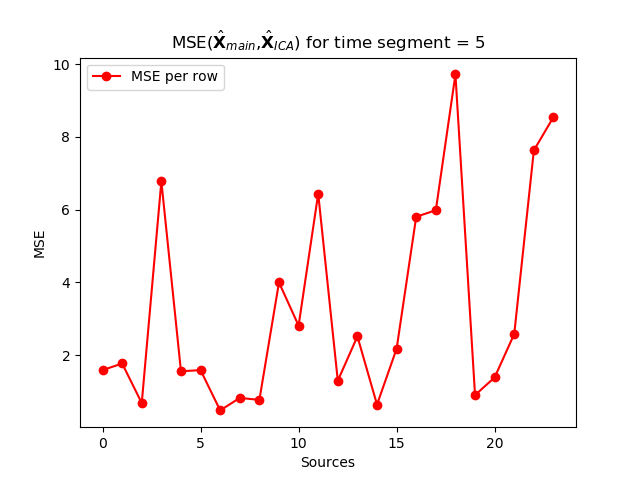
\includegraphics[width=1\linewidth]{figures/ch_7/resultat/mse_none_removed_ica_timeseg5.png}
\caption{MSE$\left(\hat{\mathbf{X}}_{\text{main}_{i}},\hat{\mathbf{X}}_{\text{ICA}_{i}}\right)$ for every row $i = 1, \dots, k$ in time segment $s=5$.}
\label{fig:M=N_2}
\end{minipage} 
\hspace{0.5cm}
\begin{minipage}[t]{.45\textwidth}
\centering
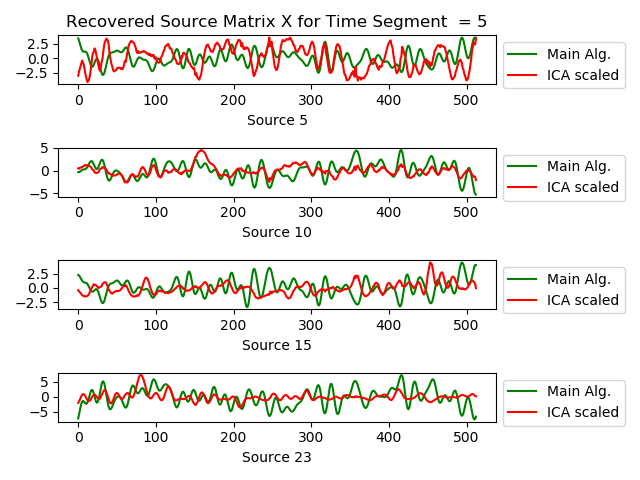
\includegraphics[width=1\linewidth]{figures/ch_7/resultat/EEG_none_removed_scaled_timeseg5S1_CClean.png}
\caption{Figure comparing four random chosen rows from $\hat{\mathbf{X}}_{\text{main}}$ and $\hat{\mathbf{X}}_{\text{ICA}}$ from time segment $s = 5$ with $M = N$ and $k=23$. Note $\hat{\mathbf{X}}_{\text{ICA}}$ is scaled for better visualization.}
	\label{fig:M=N_3}
    \end{minipage}
\end{widepage}
\end{figure}
\noindent
The test is repeated for every data set, and the results are summarized in table \ref{tab:case_0}. 
In general a low MSE is achieved in average over all segments of one data set relative to the tolerance.
And the corresponding percentage is likewise relative high, with an average at $83\%$. 
A single result is seen to deviate from the tendency, which is the data set of test subject 3 with closed eyes. 
Here a significant high average MSE value is found, indicating a majority of the segment has resulted in a significantly high MSE, while a percentage of $63\%$ was below the tolerance. 
In chapter \ref{ch:implementation} it is found that the main algorithm was capable of providing an almost exact estimate for $M = N$ when the true $\mathbf{A}$ is provided. 
Thus, it is expected that the general performance is decreased in this case where the true $\mathbf{A}$ is unknown and $\hat{\mathbf{A}}_{\text{fix}}$ is given.

The achieved results will serve as reference when analyzing the results of the following cases where the main algorithm is applied on data set with reduced number of sensors compared to the original data set.         
\begin{table}[H]
\centering
\begin{tabular}{|c|c|c|c|c|c|c|}
\hline
\multirow{2}{*}{\textbf{\begin{tabular}[c]{@{}c@{}}Case 0 \\ $M = N$\end{tabular}}} & \multicolumn{2}{c|}{Test subject 1} & \multicolumn{2}{c|}{Test subject 2} & \multicolumn{2}{c|}{Test subject 3} \\ \cline{2-7} 
                                                                                  & Open             & Close            & Open             & Close            & Open            & Close             \\ \hline
\multicolumn{1}{|c|}{Average MSE($\hat{\mathbf{X}}_{\text{ICA}},\hat{\mathbf{X}}_{\text{main}}$)}                                               & 2.913            & 5.172            & 1.572            & 15.06            & 4.753            & 19.44           \\ \hline
\begin{tabular}[c]{@{}c@{}}Segments below \\ tolerance in \%\end{tabular}          & 91             & 92            & 98 & 61             & 87            & 63 \\ \hline
\end{tabular}
\caption{Summarized results for case 0. Test is performed on the every data set.}
\label{tab:case_0}
\end{table}	
\noindent

\subsection{Case 1, $M < N$}
The main algorithm is applied on $\mathbf{Y}_s$, where the number of sensors is reduced by one-third. 
As such the main algorithm is applied on $\mathbf{Y}_s$ specified by $M = 18$ and $L_s = 516$, given $\hat{\mathbf{A}}_{\text{fix}}$ and $N = k$ provided from ICA. 
ICA is applied on the original data set with segments $\mathbf{Y}_s$ specified by $M\_ = 27$ and $L_s = 516$.  
The viewed figures correspond to those of case 0, but for the reduced number of sources $M < N$, hence detailed figure description is omitted here.   

From figure \ref{fig:M<N_1} and \ref{fig:M<N_1_2} it is seen that a majority of the segments have MSE value close to the tolerance, but the number of outliers have increased compared to case 0.
This indicates that for an increased number of segments the main algorithm do not manage to estimate enough sources sufficiently in order to stay below the tolerance. Taking the average over all segments the average achieved MSE is $5.35$.
\begin{figure}[H]
\begin{widepage}
    \begin{minipage}[t]{.45\textwidth}
		\centering
		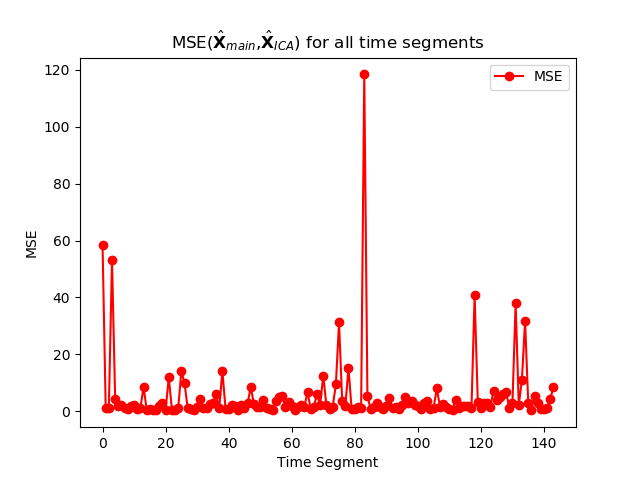
\includegraphics[width=1\linewidth]{figures/ch_7/resultat/average_mse_third_removed_ica}
	\caption{MSE$\left(\hat{\mathbf{X}}_{\text{main}},\hat{\mathbf{X}}_{\text{ICA}}\right)$ for all $n_{\text{seg}} = $ 144 segments.}
	\label{fig:M<N_1}
    \end{minipage} 
\hspace{0.5cm}
    \begin{minipage}[t]{.45\textwidth}
        \centering
		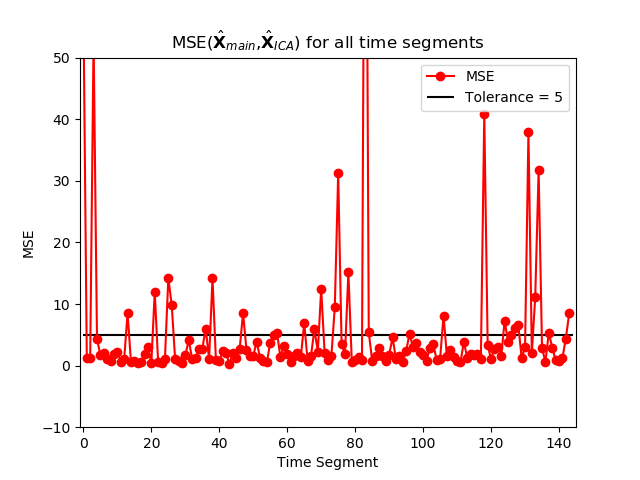
\includegraphics[width=1\linewidth]{figures/ch_7/resultat/average_mse_third_removed_ica_zoom.png}
	\caption{MSE$\left(\hat{\mathbf{X}}_{\text{main}},\hat{\mathbf{X}}_{\text{ICA}}\right)$ for all $n_{\text{seg}} = $ 144 segments. Visualized only for the y-axis interval $[-10, 50]$ for better visualization.}
	\label{fig:M<N_1_2}
    \end{minipage}
\end{widepage}
\end{figure}
\noindent 
From figure \ref{fig:M<N_2} and \ref{fig:M<N_3} showing the results of segment 5, it is seen that the MSE for each source has increased slightly compared to case 0. 
This supports the observation from figure \ref{fig:M<N_1_2}.      
\begin{figure}[H]
\begin{widepage}
    \begin{minipage}[t]{.45\textwidth}
\centering
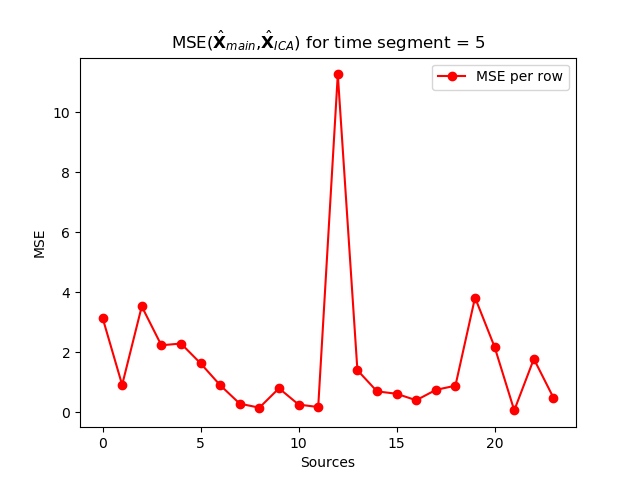
\includegraphics[width=1\linewidth]{figures/ch_7/resultat/mse_third_removed_ica_timeseg5.png}
\caption{MSE$\left(\hat{\mathbf{X}}_{\text{main}_{i}},\hat{\mathbf{X}}_{\text{ICA}_{i}}\right)$ for every row $i = 1, \dots, k$ in time segment $s=5$.}
\label{fig:M<N_2}
\end{minipage} 
\hspace{0.5cm}
\begin{minipage}[t]{.45\textwidth}
\centering
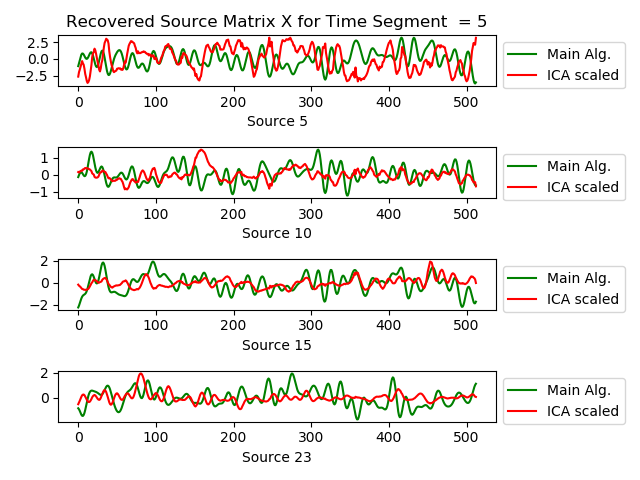
\includegraphics[width=1\linewidth]{figures/ch_7/resultat/EEG_third_removed_scaled_timeseg5S1_CClean.png}
\caption{Figure comparing four random chosen rows from $\hat{\mathbf{X}}_{\text{main}}$ and $\hat{\mathbf{X}}_{\text{ICA}}$ from time segment $s = 5$ with $M = N$ and $k=23$. Note $\hat{\mathbf{X}}_{\text{ICA}}$ is scaled for better visualization.}
	\label{fig:M<N_3}
    \end{minipage}
\end{widepage}
\end{figure}
\noindent
The test is repeated for every data set, and the results are summarized in table \ref{tab:case_1}. 
Comparing table \ref{tab:case_1} to table \ref{tab:case_0}, it is seen that the percentage of segments below the tolerance are decreasing, with the majority being close to $50\%$.
This is roughly indicating that half of the time the main algorithm do not manage to provide a sufficient estimate when $M = 2/3N$.  
Furthermore, both the average MSE and the corresponding percentages appear fluctuating relative to case 0 indicating some unreliability in the results.  
\begin{table}[H]
\centering
\begin{tabular}{|c|c|c|c|c|c|c|}
\hline
\multirow{2}{*}{\textbf{\begin{tabular}[c]{@{}c@{}}Case 1 \\ $M < N$\end{tabular}}} & \multicolumn{2}{c|}{Test subject 1} & \multicolumn{2}{c|}{Test subject 2} & \multicolumn{2}{c|}{Test subject 3} \\ \cline{2-7} 
                                                                                  & Open             & Close            & Open             & Close            & Open              & Close           \\ \hline
\multicolumn{1}{|c|}{Average MSE($\hat{\mathbf{X}}_{\text{ICA}},\hat{\mathbf{X}}_{\text{main}}$)}                                               & 9.79            & 5.351            & 13.89            & 15.13            & 6.25          & 18.21          \\ \hline
\begin{tabular}[c]{@{}c@{}}Segments below \\ tolerance in \%\end{tabular}          & 53             & 80             & 66 & 46             & 77              & 48            \\ \hline
\end{tabular}
\caption{Summarized results for case 1. Test is performed on the every data set.}
\label{tab:case_1}
\end{table}
\noindent

\subsection{Case 2, $M << N$}
The main algorithm is applied on $\mathbf{Y}_s$, where the number of sensors is reduced to half. 
As such the main algorithm is applied on $\mathbf{Y}_s$ specified by $M = 13$ and $L_s = 516$, given $\hat{\mathbf{A}}_{\text{fix}}$ and $N = k$ provided from ICA.  
ICA is applied on the original data set with segments $\mathbf{Y}_s$ specified by $M\_= 27$ and $L_s = 516$. 
The viewed figures correspond to those of case 0 and case 1, but for further reduce number of sources $M << N$, hence detailed figure description is omitted.   

From figure \ref{fig:M<<N_1} and \ref{fig:M<<N_1_2} it is seen that the MSE value for each segment is more widely scatted around the tolerance, compared to case 0 and 1. 
Outliers, where the MSE value has increased significantly, do also occur similar to case 1. 
This indicates that the performance of the main algorithm has decreased further, compared to case 1. Taking the average over all segments the average achieved MSE is $11.36$.
\begin{figure}[H]
\begin{widepage}
    \begin{minipage}[t]{.45\textwidth}
		\centering
		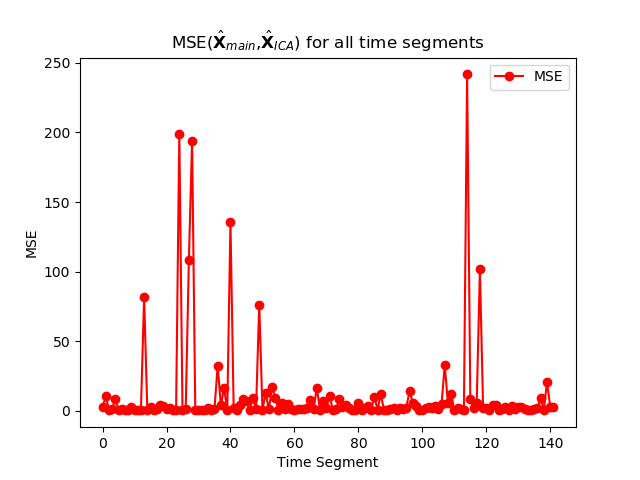
\includegraphics[width=1\linewidth]{figures/ch_7/resultat/average_mse_second_removed_ica}
	\caption{MSE$\left(\hat{\mathbf{X}}_{\text{main}},\hat{\mathbf{X}}_{\text{ICA}}\right)$ for all $n_{\text{seg}} = $ 144 segments.}
	\label{fig:M<<N_1}
    \end{minipage} 
\hspace{0.5cm}
    \begin{minipage}[t]{.45\textwidth}
        \centering
		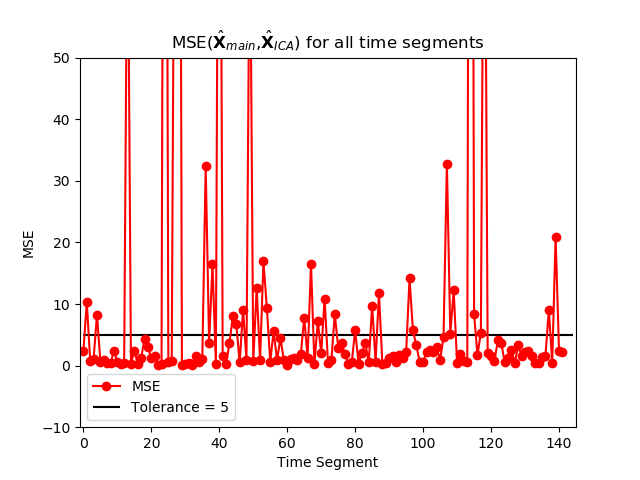
\includegraphics[width=1\linewidth]{figures/ch_7/resultat/average_mse_second_removed_ica_zoom.png}
	\caption{MSE$\left(\hat{\mathbf{X}}_{\text{main}},\hat{\mathbf{X}}_{\text{ICA}}\right)$ for all $n_{\text{seg}} = $ 144 segments. Visualized only for the y-axis interval $[-10, 50]$ for better visualization.}
	\label{fig:M<<N_1_2}
    \end{minipage}
\end{widepage}
\end{figure}
\noindent 
The above indication is supported by figure \ref{fig:M<<N_2} and \ref{fig:M<<N_3} showing an general increase in MSE. 
However, segment 5 makes a fairly good example as the majority of the sources have achieves a MSE below the tolerance of 5. 
From figure \ref{fig:M<<N_3} the increased MSE do not appear visually compared to either case 1 or case 0.        
\begin{figure}[H]
\begin{widepage}
    \begin{minipage}[t]{.49\textwidth}
\centering
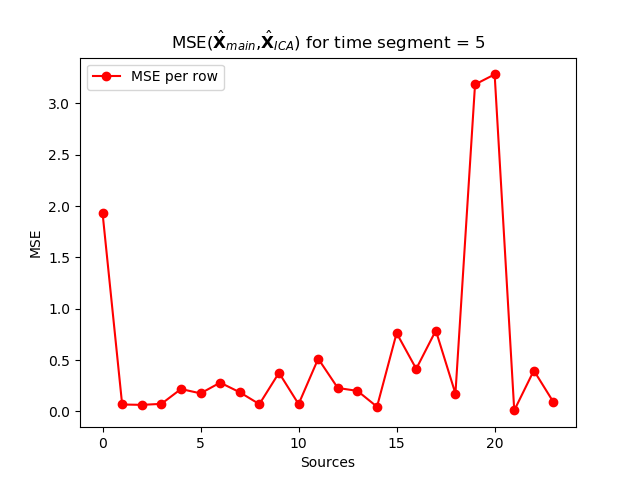
\includegraphics[width=1\linewidth]{figures/ch_7/resultat/mse_second_removed_ica_timeseg5.png}
\caption{MSE$\left(\hat{\mathbf{X}}_{\text{main}_{i}},\hat{\mathbf{X}}_{\text{ICA}_{i}}\right)$ for every row $i = 1, \dots, k$ in time segment $s = 5$.}
\label{fig:M<<N_2}
\end{minipage} 
\hspace{.5cm}
\begin{minipage}[t]{.49\textwidth}
\centering
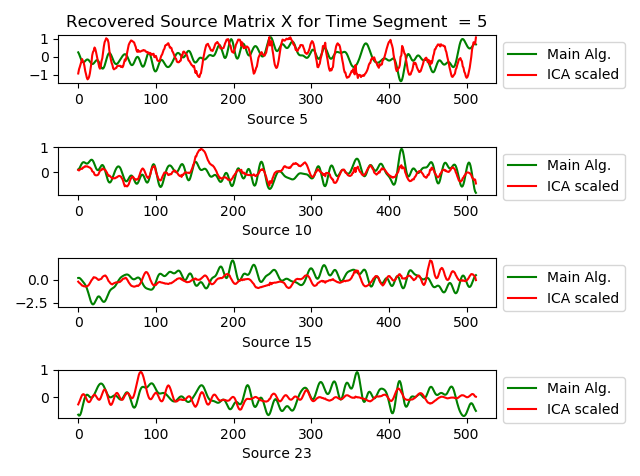
\includegraphics[width=1\linewidth]{figures/ch_7/resultat/EEG_second_removed_scaled_timeseg5S1_CClean.png}
\caption{Figure comparing four random chosen rows from $\hat{\mathbf{X}}_{\text{main}}$ and $\hat{\mathbf{X}}_{\text{ICA}}$ from time segment $s = 5$ with $M << N$ and $k=23$. Note $\hat{\mathbf{X}}_{\text{ICA}}$ is scaled for better visualization.}
	\label{fig:M<<N_3}
    \end{minipage}
\end{widepage}
\end{figure}
\noindent
The test is repeated for every data set, and the results are summarized in table \ref{tab:case_2}. Comparing table \ref{tab:case_0} to table \ref{tab:case_1} it is generally seen that the percentage of segments below the tolerance are not decreased but improved.
Though, without getting close to the tendency from case 0. 
Furthermore, the average MSE have not increased remarkably compared to case 1. 
As such the performance of the main algorithm in case 2 is in general not found to be worse than for case 1.
However, a clear improvement is not seen either.  
\begin{table}[H]
\centering
\begin{tabular}{|c|c|c|c|c|c|c|}
\hline
\multirow{2}{*}{\textbf{\begin{tabular}[c]{@{}c@{}}Case 2\\ $M << N$\end{tabular}}} & \multicolumn{2}{c|}{Test subject 1} & \multicolumn{2}{c|}{Test subject 2} & \multicolumn{2}{c|}{Test subject 3} \\ \cline{2-7} 
                                                                                  & Open             & Close            & Open             & Close            & Open             & Close            \\ \hline
\multicolumn{1}{|c|}{Average MSE($\hat{\mathbf{X}}_{\text{ICA}},\hat{\mathbf{X}}_{\text{main}}$)}                                               & 8.378            & 11.36            & 19.58            & 13.11            & 13.99           & 11.96            \\ \hline
\begin{tabular}[c]{@{}c@{}}Segments below \\ tolerance in \%\end{tabular}          & 75             & 74             & 42 & 72             & 69             & 69 \\ \hline
\end{tabular}
\caption{Summarized results for case 2. Test is performed on the every data set.}
\label{tab:case_2}
\end{table}
\noindent


\subsection{Summary of Results}
The main algorithm have been tested on 6 data sets of EEG measurement, for a varying relation between the number of sensors and sources -- respectively case 0, 1 and 2.
When the number of sensors is reduced with respect to the number of sources to be found, a significant decrease in performance was found -- comparing case 0 and 1. 
However a corresponding decrease of performance was not found when further sensors was removed -- comparing case 1 and 2. 

From the conclusions made in chapter \ref{ch:implemantation} it was not expected that the main algorithm would provide successful results, without estimating $\textbf{A}$ form the data. 
The results of case 0 do however indicate a solid estimate provided by the main algorithm, with an average percentage of successfully estimated segments at $83\%$. 

Furthermore it is worth to note that the resulting MSE values has potential for improvement when considering optimization of the source localisation of the ICA estimate, cf. appendix \ref{app:ica_test}.


\section{Alpha Wave Analysis}\label{sec:alpha_test}
As mentioned in chapter \ref{ch:motivation} brain signals can be classified into four groups according to the dominant frequency \cite{EEGsignalprocessing}. 
It is known that when a person closes the eyes, when relaxing, the amount of alpha frequency raises and become the dominant frequency. 
The provided EEG measurements consist of measurements from a test subject with both open and closed eyes.
Hence, it would be interesting to investigate this relation between the alpha frequency for open and closed eyes. 
The interesting part is then to compare the relation achieve from the provided EEG measurements and the sources signals estimated by the main algorithm.

With a test of this kind, it is possible to evaluate the recovered source signals from a different perspective. 
Here the objective is first of all to see the behavior with respect to the frequency, expected by the theory. 
Next it is interesting to investigate the aspect of analysis performed on EEG level versus analysis performed on source level, as discussed in chapter \ref{ch:motivation}.              

\subsection{Test Setup}
For this comparison the data sets of test subject 1, \texttt{S1\_OClean} and \texttt{S1\_CClean}, EEG measurements of open and closed eyes respectively, will be used. 
It is expected that the power within the alpha frequency band is highest for the closed eyes data set, \texttt{S1\_CClean}.
To compare the amount of alpha frequency in the two data sets, a bandpass filter is used to isolate the alpha frequencies. 
To perform the filtering a bandpass Butterworth filter of order 5 with cut-off frequencies $8$ Hz and $13$ Hz will be applied. 
The filtering is performed in the time domain to both the EEG signals and the source signals recovered from the main algorithm.
The filtering process is illustrated in figure \ref{fig:dft_1}.
In the illustrated example only one source signal is investigated in both time and frequency domain, where the fast Fourier transformation (FFT) is applied \cite[Chapter 9]{FFT}. 
The source signal of interest was recovered within the closed eyes data set \texttt{S1\_CClean} from time segment $15$. 
The system specification used to recover the source signal was $M = 27$ and $k = 14$, with $k$ obtained by ICA.
\begin{figure}[H]
\centering
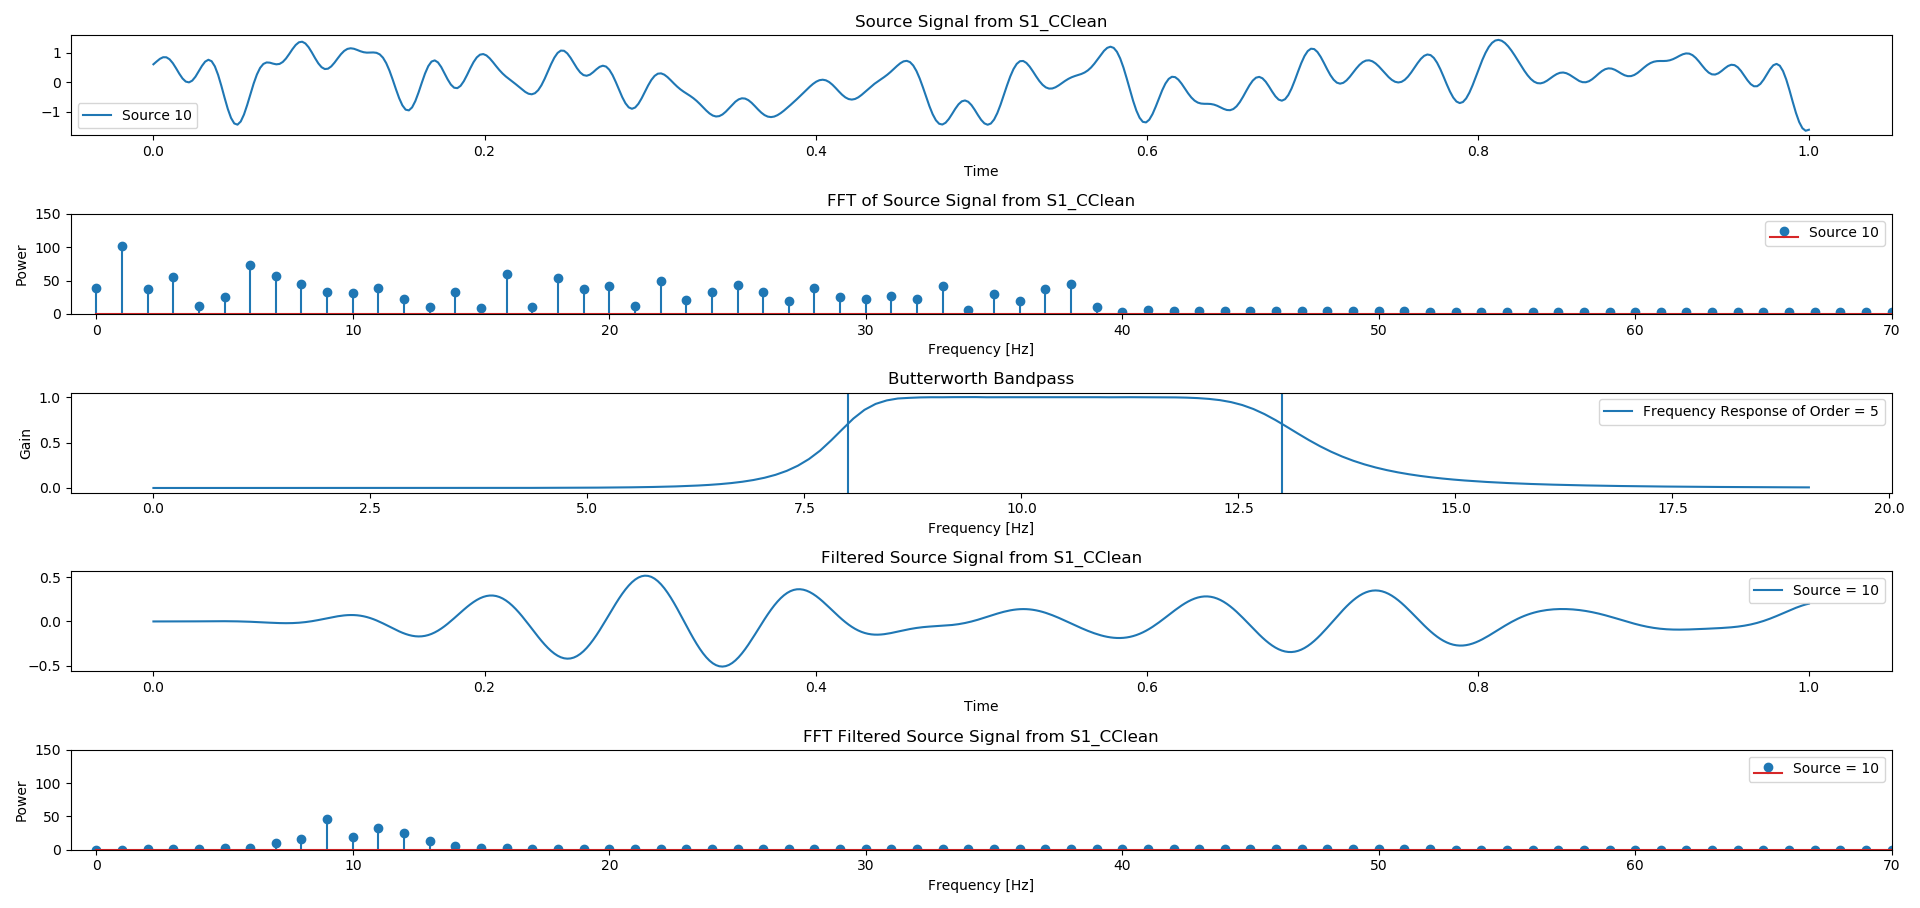
\includegraphics[scale=0.28]{figures/ch_7/DFT_plot_X_timeseg15_source10.png}
\caption{Time domain and frequency plot of a recovered source signal, filtered and non-filtered, from the time segment 15.}
\label{fig:dft_1}
\end{figure}
\noindent
The first plot in figure \ref{fig:dft_1} is the recovered source signal in the time domain. 
The next plot is the same source signal but transformed to the frequency domain by the FFT. 
The plot has been scaled to only show the frequencies from 0-70 Hz and the power from 0 to 150. 
The third plot illustrates the frequency response of the bandpass Butterworth filter with order 5. 
The vertical blue lines illustrate the cut-off frequencies at 8 Hz and 13 Hz.
Plot number four is the recovered source signal filtered by the bandpass Butterworth filter, plotted in the time domain. 
The last plot is the filtered source signal plotted in the frequency domain. 
This verifies that the signal of interest has been filtered according to the alpha band. 
From the filtered source signal in the time domain, the signal resemble the alpha wave as seen in figure \ref{fig:EEG_example}.

The filtering process is applied to 100 time segments of both the closed eyes and open eyes for respectively the EEG measurements and the recovered source signals. 
Note that for each time segment all present source signals or sensor measurements have been summed such that only one signal resembles each time segment.
Then for each time segment the relation between closed and open eyes is computed, with respect to power within the alpha band. 
The relation is defined as 
\begin{align*}
\text{Relation} = \frac{C}{O}, 
\end{align*}
where $C$ is the average power from closed eyes, and $O$ is the average power from the open eyes segment. 
This is done for both the EEG measurements and the recovered source signals. 
By this it is possible to compare the relation found on source level and the relation seen on EEG level.  

\subsection{Results}
Figure \ref{fig:dft_2} shows an example of one time segment. 
To the left is the power spectrum of the filtered EEG measurements visualized for open and closed eyes respectively. 
The resulting relation between the two is $1.15$. 
To the right is the power spectrum of the filtered source signals. 
Likewise for open and closed eyes respectively. 
The resulting relation between open and closed eyes is here $1.41$.  
\begin{figure}[H]
\centering
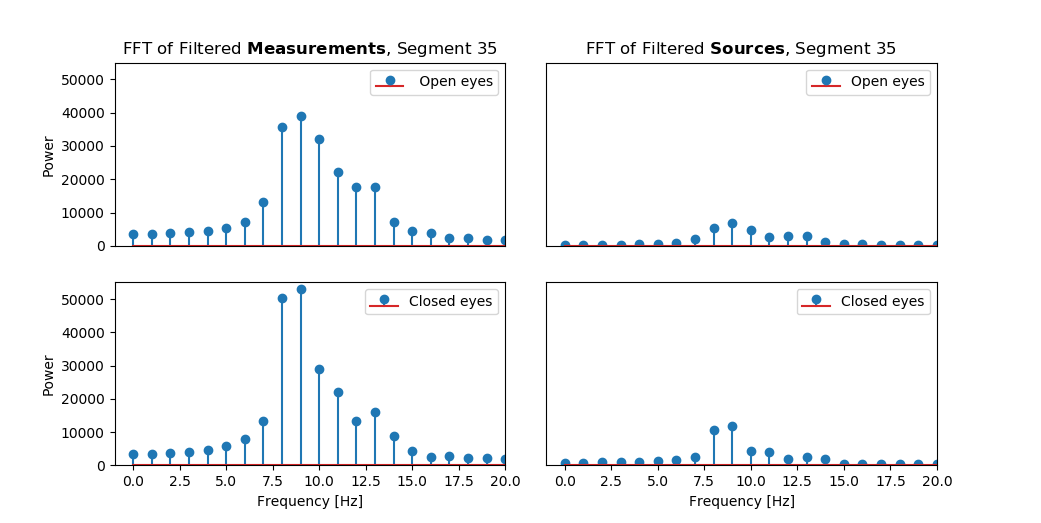
\includegraphics[scale=0.5]{figures/ch_7/FFT_plot.png}
\caption{Power spectrum of the filtered EEG measurements and recovered source signals of time segment 35 for open and closed eyes data set of test subject 1.}
\label{fig:dft_2}
\end{figure}
\noindent
By observing figure \ref{fig:dft_2} it is seen, for the specific segment, that the power within the alpha band is significantly larger within the EEG measurements compared to the sources. 
Furthermore, is it seen for both the EEG measurements and the source signals that the power has increased from open to closed eyes. 
Considering the calculated relations is it seen that the biggest increase in power is found on source level. 
This behavior does support the theory, however the result of a single segment is not sufficient to draw any conclusion.          

Figure \ref{fig:dft_5} and \ref{fig:dft_6} illustrate the $C/O$ relation computed for the 100 time segments, of the EEG measurements and source signals respectively. 
The horizontal line in the plots marks the 1/1 relation.
As such the segments where the highest power was found for closed eyes lies above the line - supporting the theory. Opposite the segments with least power found for closed eyes lies below the line.      
\begin{figure}[H]
\begin{widepage}
    \begin{minipage}[t]{.49\textwidth}
\centering
\includegraphics[width=1\linewidth]{figures/ch_7/DFT_Y_Difference.png}
\caption{The $C/O$ relation for EEG measurements for 100 time segments. The average $C/O$ over all segments is $1.16$.}
\label{fig:dft_5}
\end{minipage} 
\hspace{.5cm}
\begin{minipage}[t]{.49\textwidth}
\centering
\includegraphics[width=1\linewidth]{figures/ch_7/DFT_X_Difference.png}
\caption{The $C/O$ relation of source signals for 100 time segments. The average $C/O$ over all segments is $2.01$.}
	\label{fig:dft_6}
    \end{minipage}
\end{widepage}
\end{figure}
\noindent
From the figures it is clear the behavior seen from the example of segment 35, is not a continuous behavior. 
It is seen both on EEG level and source level that relation scatters around the horizontal line, indicating that the relation is not stationary over time.  
On figure \ref{fig:dft_6} is it seen that the $C/O$ relation range from near zero to beyond 20 for a few segments, indicating a significant change in power compared to figure \ref{fig:dft_5}. 
With 57 out of 100 segments lying below the horizontal line the behavior is considered more or less random. 
From these observations the expected behavior was not found. 
This does support the earlier findings with respect to the main algorithm, indicting a significant unreliability to the result. 

With respect to the method for computing the $C/O$ relation it could be considered whether computing the relation for every segment is the right choice. 
One could argue that summing the power over all segments for respectively open and closed eyes and then compute the $C/O$ relation would yield a different result.  


